\documentclass{article}

% if you need to pass options to natbib, use, e.g.:
%     \PassOptionsToPackage{numbers, compress}{natbib}
% before loading neurips_2019

% ready for submission
% \usepackage{neurips_2019}

% to compile a preprint version, e.g., for submission to arXiv, add add the
% [preprint] option:
%     \usepackage[preprint]{neurips_2019}

% to compile a camera-ready version, add the [final] option, e.g.:
     \usepackage[final]{conducktors}

% to avoid loading the natbib package, add option nonatbib:
%     \usepackage[nonatbib]{neurips_2019}

\usepackage[utf8]{inputenc} % allow utf-8 input
\usepackage[T1]{fontenc}    % use 8-bit T1 fonts
\usepackage{hyperref}       % hyperlinks
\usepackage{url}            % simple URL typesetting
\usepackage{booktabs}       % professional-quality tables
\usepackage{amsfonts}       % blackboard math symbols
\usepackage{nicefrac}       % compact symbols for 1/2, etc.
\usepackage{microtype}      % microtypography
\usepackage[pdftex]{graphicx}
\usepackage{subcaption}

\title{Duckietown - Reinforcement Learning based on World Models\\ \textit{Duckietown - megerősítéses tanulás a World Models alapján}}

% The \author macro works with any number of authors. There are two commands
% used to separate the names and addresses of multiple authors: \And and \AND.
%
% Using \And between authors leaves it to LaTeX to determine where to break the
% lines. Using \AND forces a line break at that point. So, if LaTeX puts 3 of 4
% authors names on the first line, and the last on the second line, try using
% \AND instead of \And before the third author name.

\author{%
  conDUCKtors\\
  \textit{Máté Büki, Péter Zoltán Sánta, Gábor Tamás}\\
  Deep Learning in Practice with Python and LUA\\
  VITMAV45\\
  Budapest University of Technology and Economics \\
  2019/20/1
  %\texttt{hippo@cs.cranberry-lemon.edu} \\
  % examples of more authors
  % \And
  % Coauthor \\
  % Affiliation \\
  % Address \\
  % \texttt{email} \\
  % \AND
  % Coauthor \\
  % Affiliation \\
  % Address \\
  % \texttt{email} \\
  % \And
  % Coauthor \\
  % Affiliation \\
  % Address \\
  % \texttt{email} \\
  % \And
  % Coauthor \\
  % Affiliation \\
  % Address \\
  % \texttt{email} \\
}

\begin{document}

\maketitle

\begin{abstract}
In our homework, we use a reinforcement learning framework to teach an agent to be able to follow the lane in the Duckietown Gym environment. The model our work is based on was named World Models \cite{worldmodels} and was published in 2018. The main idea of the model is to use a compressed representation of the observable environment instead of the raw image seen by the agent. The transformed observations are then passed to a recurrent neural network, which is responsible for the prediction of the next observation. Finally, the agent is trained using reinforcement learning. We have modified the model to use the so called SAC policy instead of a simple linear function in the RL phase of the training, which made the RNN part of the model unnecessary.\newline

\textit{Házi feladatunk keretein belül egy megerősítéses tanulás alapú modellt használva tanítottunk egy ágenst arra, hogy képes legyen az út követésére a Duckietown Gym szimulációs környezetben. Ehhez munkánk során a 2018-ban publikált ún. World Models \cite{worldmodels} modellt használtuk kiindulási alapként. A modell különlegessége, hogy nem az ágens által látott környezet nyers képét használja fel, hanem a környezet egy tömörített reprezentációját. Az így kapott, már transzformált megfigyeléseket továbbítja egy rekurrens neurális hálónak, amelynek feladata, hogy az ágens által a következő lépés során látott környezet transzformált formáját prediktálja. Végül az ágens megerősítéses tanulás segítségével tanul. Az eredeti modellt úgy módosítottuk, hogy az eredeti cikkben szereplő lineáris függvény helyett az ún. SAC policy-t használtuk a megerősítéses tanulás során, így az RNN-nek már nem volt létjogosultsága.}
\end{abstract}

%%%%%%%%%%%%%%%%%%%%%%
\section{Introduction}
%%%%%%%%%%%%%%%%%%%%%%

Many of the algorithms in the field of artifical intelligence are inspired by how humans learn and think. Our brain is able to learn an abstract representation of the information it gets from our environment. Our homework is based on a model called World Models \cite{worldmodels}, which mimics this behaviour. In their article, the authors present a new framework for facilitating the policy evolution in a reinforcement learning \cite{rl} task. The main idea of their work is that they transform the environment seen by the agent into a so called latent vector, and the reinforcement learning algorithm is trained using the already transformed reality. So the agent learns in its own world, hence the name of the model. It is important to note that the idea of using a VAE network together with an evolutional reinforcement learning algorithm is not unique, there is an article \cite{vae_es} published in 2017 that already using this idea.


%%%%%%%%%%%%%%%%%%%%%
\section{Agent model}
%%%%%%%%%%%%%%%%%%%%%


Our task was to implement the World Models\cite{worldmodels} (that has been already done for the OpenAI CarRacing environment) for the Duckietown Gym environment. In this chapter we briefly introduce the architecture of the model.

World Models has 3 basic components, depicted in figure \ref{fig:model}.

\begin{figure}
    \centering
    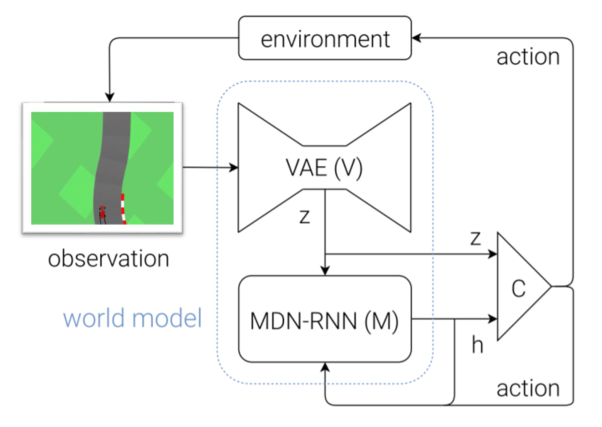
\includegraphics[width=0.55\textwidth]{world_models.png}
    \caption{Components of World Models}
    \label{fig:model}
\end{figure}

\subsection{Vision (V)}

The Vision model is a simple Convolutional Variational Autoencoder (VAE) \cite{vae1}, \cite{vae2} which takes an observation (2D image) from the environment and encodes it into a latent vector $z$ of size 32.

The architecture of the VAE network is shown in figure \ref{fig:vae}.

\subsection{MDN-RNN (M)}

The second building block of the model is an LSTM-based \cite{lstm} recurrent neural network which is combined with a mixture density network\cite{MDN}. It takes the latent vector $z$ from the vision module, the previous action $a$ chosen by the controller and the previous hidden state $h$ of itself. Similarly to the vision module, its goal is to capture a latent understanding/observation of the environment by predicting what would the next $z$ look like.

The architecture of the Memory RNN network is shown in figure \ref{fig:rnn}.

\begin{figure}[!ht]
    \centering
    \begin{subfigure}[b]{.45\textwidth}
        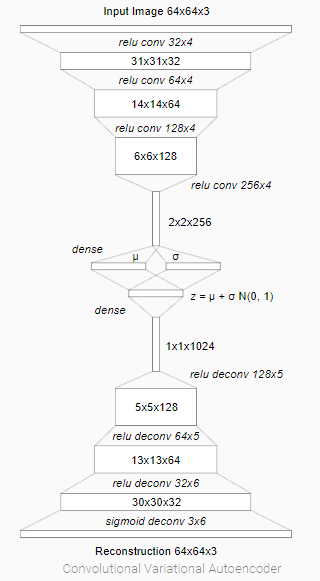
\includegraphics[width=\textwidth]{VAE.png}
        \caption{VAE}
        \label{fig:vae}
    \end{subfigure}
    \begin{subfigure}[b]{.54\textwidth}
        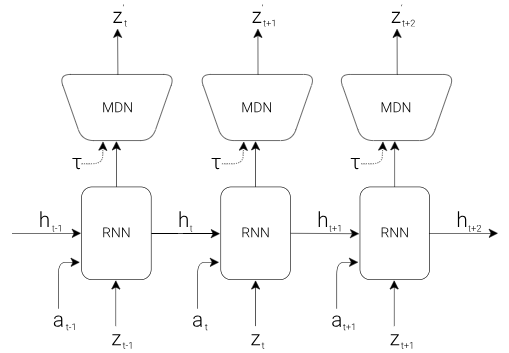
\includegraphics[width=\textwidth]{RNN.png}
        \caption{Memory RNN}
        \label{fig:rnn}
    \end{subfigure}
    \caption{Architecture of the given components}
    \label{fig:architecture}
\end{figure}

\subsection{Controller (C)}
In their implementation, the authors used the Covariance-Matrix Adaptation Evolution Strategy
(CMA-ES) \cite{cma}.

The controller consists of a simple single layer linear model which maps the vision module’s observation $z$ and the memory module’s hidden state $h$ to an action $a$ at each time step. The output is an action-vector (numpy array) of size 2 containing the quantitative representation of the velocity [-1.0 to 1.0] and the angle of the steering wheel [-1.0 to 1.0].


%%%%%%%%%%%%%%%%%%%%%%%%
\section{Implementation}
%%%%%%%%%%%%%%%%%%%%%%%%


In our homework, we used the Duckietown Gym \cite{gym_duckietown} environment. Gym \cite{gym} is a toolkit for developing and comparing reinforcement learning algorithms. It supports teaching agents everything from walking to playing games like CarRacing or Pacman. Duckietown is a playful learning experience for state-of-the-art robotics and AI. It makes it possible to develop and test autonomous driving algorithms with Deep Learning in a joyful sandbox environment. To make the development easier, the Duckietown Foundation published the Duckietown Simulator based on the OpenAI Gym environment.

Our goal was to modify an already existing PyTorch implementation of World Models\footnote{https://github.com/ctallec/world-models} so that we can apply it for Gym-Duckietown.

\subsection{Modified agent model}

\subsubsection{Vision (V)}
We had to modify the architecture of the VAE due to the fact that the resolution of the images extracted from the Duckietown Gym environment is different (much larger) compared to the CarRacing environment. Additionally, we changed the size of the latent vector from 32 to 64, since we had to store more information in it.\\
We performed three different modifications in the following order: firstly we supplemented the VAE network with several convolutional and deconvolutional layers. Thanks to this it was able to encode and decode images with resolution of 480x640. Secondly, we put batchnorm layers between each and every already existing layer. Thirdly, we put in the network several more layers which didn't modify the spatial dimensions of the feature maps being propagated through the network. The number of input channels of these layers equaled the number of output channels.

\subsubsection{MDN-RNN (M)}
Since we have modified the controller as described below, it was not clear for us how we could combine the MDN-RNN and our new controller. An important difference compared to the CarRacing-based implementation is that they had the current observation and the proposed action, while what we have is the last action and the observation after that. We came to the conclusion that we have to exclude the RNN model from our implementation.

\subsubsection{Controller (C)}
Instead of the simple linear model, we used the so called SAC reinforcement learning policy \cite{sac}.

An AC model in general uses a Q-network to estimate the Q function. Given a sample, the neural network predicts a Q value for every possible action. The weights of the Q network are updated using SGD and backpropagation. A stack of consecutive frames is used as a representation of a single input.

SAC uses entropy regularization and is trained to maximize a trade-off between expected return and entropy. Entropy is used to describe the randomness in the policy. A higher value of entropy leads in more exploration, which can accelerate the learning process.

\subsection{Data preparation}
We have created a dataset of 100 training, 50 testing and 20 validation rollouts. A rollout consists of four arrays (compressed in .npz files) containing the values returned by the step function which is involved in the Gym environment class. The images given by step() are located in "observations".

\subsection{Training the model}
We made the starting position of our agent fixed, which makes the training easier and faster. We used the so called ''udem1'' map.

Since our model has two components, we had to train it sequentially. In the first step, the VAE network was trained independently in the following way:
\begin{enumerate}
    \item The network takes an image with a size of (640 x 480 x 3) as an input.
    \item A convolutional network creates a so called $z$ vector of length 64 as a compressed representation of the input image.
    \item A deconvolutional network then takes the $z$ vector as input and generates a (640 x 480 x 3) sized image as an output.
    \item Finally, the VAE network computes the loss based on the similarity of the input (original) and the output (generated) images. If the two images are quite similar, that means that the VAE learned to compress images efficiently into a vector of length 64.
\end{enumerate}

Note that the deconvolutional network will only be used during training, after that it will be ''deactivated''. Before going further, we will first fix the parameters of the VAE (we do not want it to train any more).

The controller takes the $z$ vector (length: 64) from the VAE, and using the SAC policy, generates an action $a$ as an output. Based on the action of the controller, the environment generates a reward (a float number) that indicates how good decision the controller has made. The aim of the controller is to maximize the reward it gets.

We use wrappers for modifying the default behaviour of the Duckietown Gym environment. The action wrapper overrides the default shape of the action, so that it tells the SAC that we expect three floating point numbers between 0 and 1. We find the maximum value in this array, and based on its position (1st, 2nd or 3rd) we define the direction of our next discrete step (left, right, straight respectively). The reward wrapper - according the studies carried out earlier - can optimise the way the reward is computed by the environment. The observation wrapper passes the action produced by the SAC (which creates its action using the action wrapper) through the step function of the Gym environment, and transforms the raw image using the VAE into a latent vector.


%%%%%%%%%%%%%%%%%%%%%%%
\subsection{Evaluation}
%%%%%%%%%%%%%%%%%%%%%%%

\subsubsection{VAE}
For evaluating the performance of image encoding and decoding we used the quantity called Intersection of Unions (IoU). This is related to the ratio of the number of appropriately decoded pixels and the number of all pixels. We computed the average number of pixels which completely matched with the encoded and decoded ones. We found that there were 23 pixels out of 1201 test images that satisfied this condition the average IoU was accordingly 0,019. We used a channelwise method as well to compute the IoU, this computation gave IoU values for the R, G and B channels 0.6953, 0.8793 and 0.0092 respectively.

\begin{figure}[!ht]
    \centering
    \begin{subfigure}[b]{.24\textwidth}
        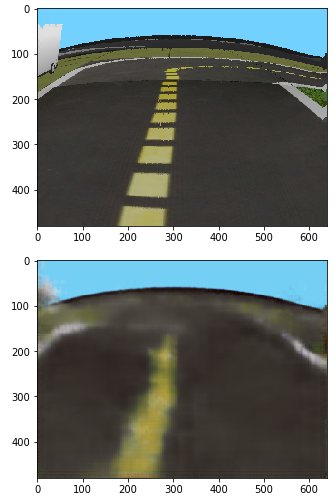
\includegraphics[width=\textwidth]{vae1.png}
    \end{subfigure}
    \begin{subfigure}[b]{.24\textwidth}
        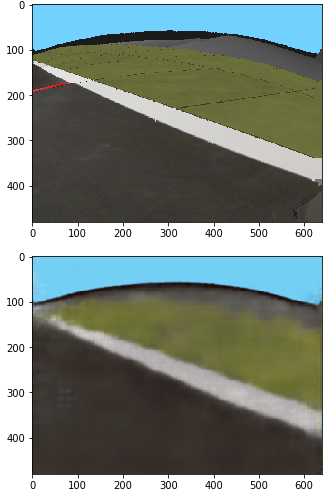
\includegraphics[width=\textwidth]{vae2.png}
    \end{subfigure}
    \begin{subfigure}[b]{.24\textwidth}
        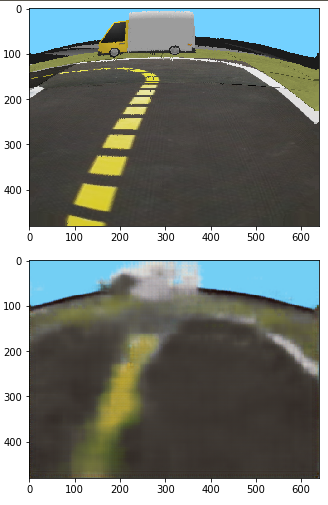
\includegraphics[width=\textwidth]{vae3.png}
    \end{subfigure}
    \begin{subfigure}[b]{.24\textwidth}
        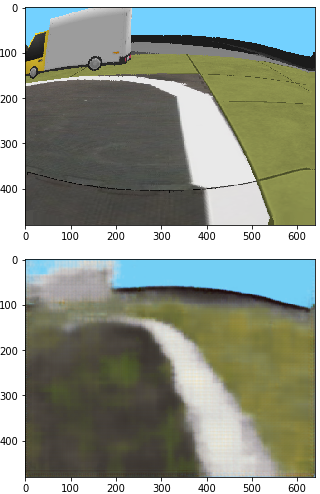
\includegraphics[width=\textwidth]{vae4.png}
    \end{subfigure}
    \caption{Examples of how our trained VAE is able to encode, and then decode a given observation from the Duckietown Gym environment.}
    \label{fig:trained_vae}
\end{figure}

\subsubsection{Controller}
During the testing phase, we switch of the Critic part of the SAC, and the Actor is in eval mode, which means that it produces actions that we can observe in the Duckietown Gym environment.

The Controller has been trained for 150000 steps. The result is an agent, which is able to follow the road and to stay on the right lane.


%%%%%%%%%%%%%%%%%
\section{Summary}
%%%%%%%%%%%%%%%%%
All in all, we can say that the policy learnt by the controller is acceptable. However, additional work is needed to optimise the components of our model in order to be able to give a better result.


\subsubsection*{Acknowledgments}

We wish to acknowledge the help provided by Róbert Moni, who has guided us throughout the semester.

\subsubsection*{Contributions}
All of us participated in discovering the literature and reading the papers we required to proceed. In the beginning, we worked together to understand the World Models. This means we have created our first training dataset, and created and trained the first version of our VAE network together. In the early stages of the project, we experimented with the RNN together. As the final deadline came closer, we divided the tasks. The hyperparameter optimization of the VAE was done by Máté Büki. The Controller was implemented and fine-tuned by Péter Zoltán Sánta. Rollout generation was Gábor Tamás's responsibility. In the end, we documented our work together. During the semester, we tried to work as collaboratively as possible to ensure all of us can learn as much as possible.



\small
\bibliographystyle{ieeetr}
\bibliography{refs}

\end{document}